\begin{resumen}

% Insertando imagen.
  \begin{figure}[!htb]
  \centering
  \subfloat{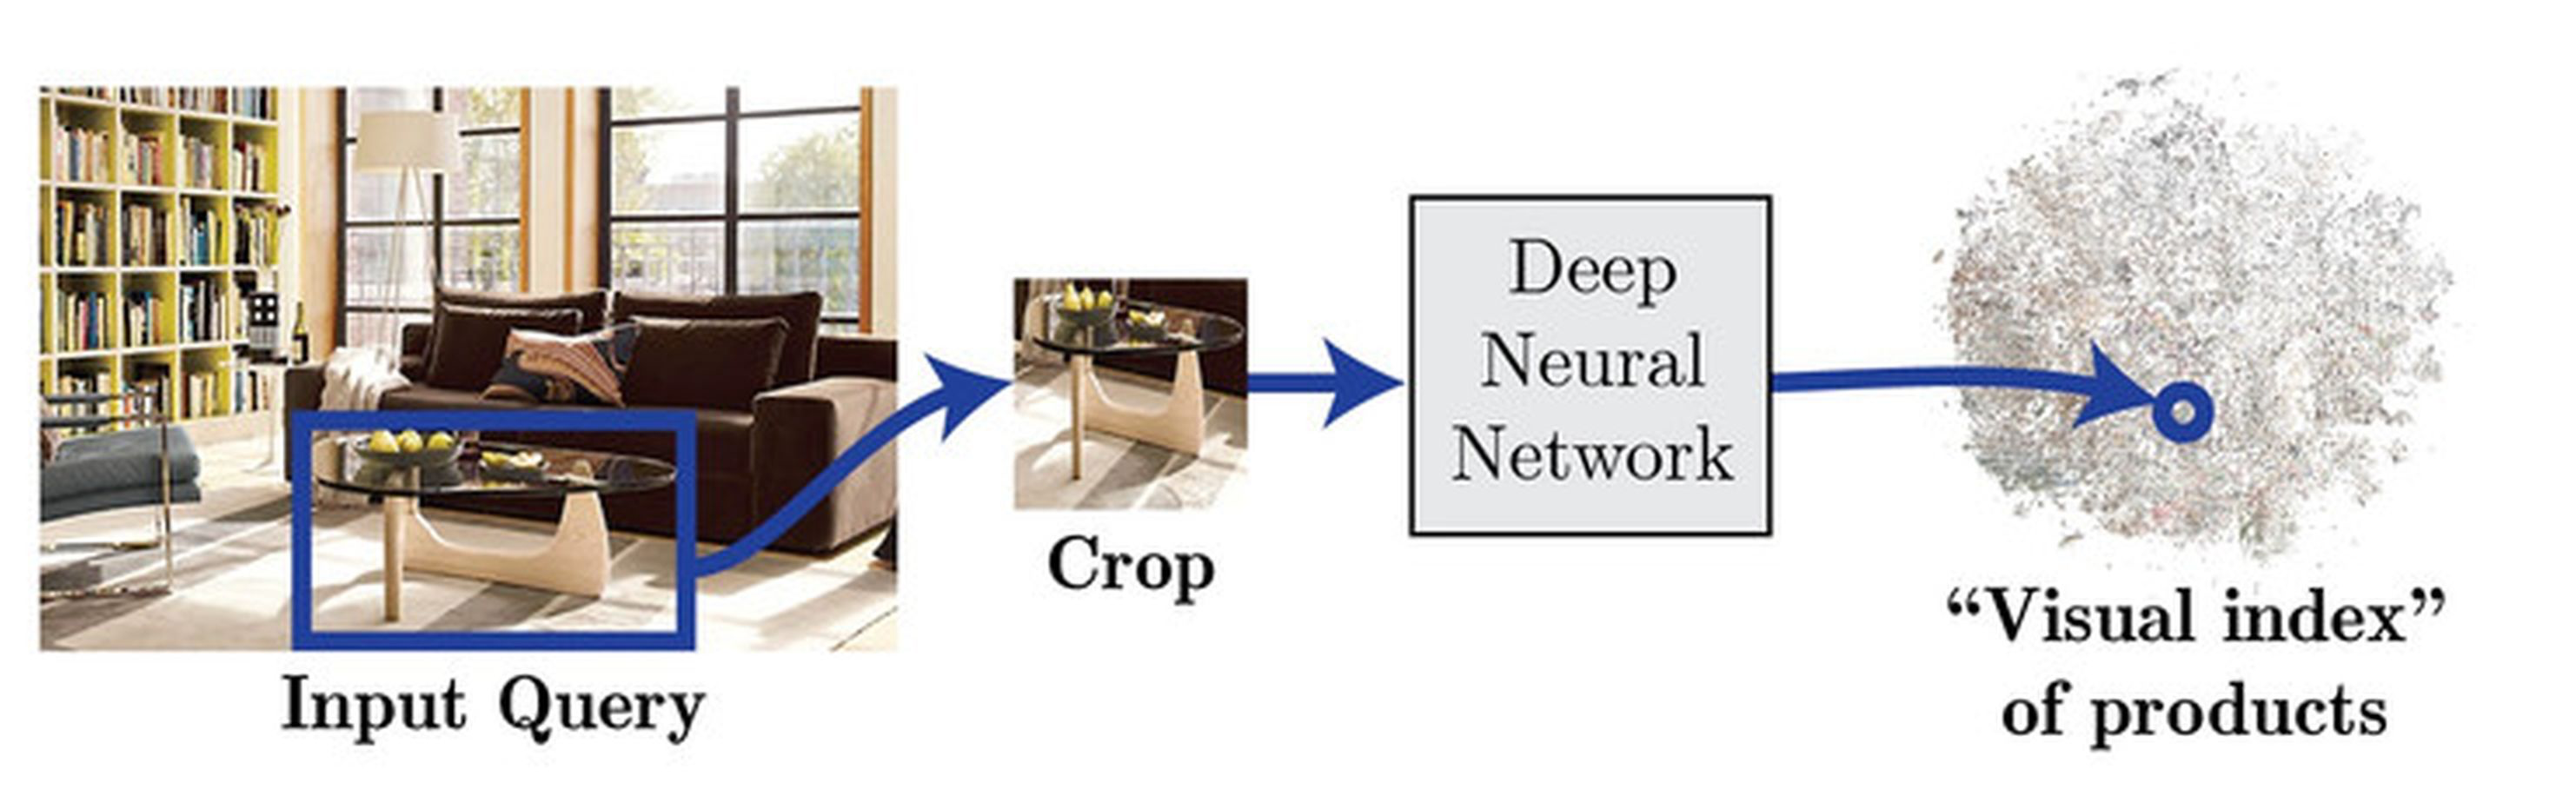
\includegraphics[width=5.7in]{graficos/Abstract}}
  \label{fig:Attrib2}
  \end{figure}
% Fin de figura MOdificado

Aquí deberas colocar entre 100 y 150 palabras como máximo, el problema que intentas resolver, la justificación y los aportes o soluciones que planteas.

\begin{flushleft}
\textbf{Palabras clave:} Inteligencia artificial, Programación paralela, Procesamiento de videos.
\end{flushleft}

\end{resumen}
